\documentclass[UTF8,a4paper,10pt, twocolumn]{ctexart}
\usepackage[left=2.50cm, right=2.50cm, top=2.50cm, bottom=2.50cm]{geometry}

% -- text font --
% compile using Xelatex

%\setmainfont{Microsoft YaHei}  % 微软雅黑
%\setmainfont{YouYuan}  % 幼圆
%\setmainfont{NSimSun}  % 新宋体
%\setmainfont{KaiTi}    % 楷体
%\setmainfont{SimSun}   % 宋体
%\setmainfont{SimHei}   % 黑体

\usepackage{times}
%\usepackage{mathpazo}
%\usepackage{fourier}
%\usepackage{charter}
%\usepackage{helvet}

\usepackage{amsmath, amsfonts, amssymb} % math equations, symbols
\usepackage[english]{babel}
\usepackage{color}      % color content
\usepackage{graphicx}   % import figures
\usepackage{url}        % hyperlinks
\usepackage{bm}         % bold type for equations
\usepackage{multirow}
\usepackage{booktabs}
\usepackage{epstopdf}
\usepackage{epsfig}
\usepackage{algorithm}
\usepackage{algorithmic}
\renewcommand{\algorithmicrequire}{ \textbf{Input:}}     % use Input in the format of Algorithm
\renewcommand{\algorithmicensure}{ \textbf{Initialize:}} % use Initialize in the format of Algorithm
\renewcommand{\algorithmicreturn}{ \textbf{Output:}}     % use Output in the format of Algorithm

\usepackage{fancyhdr}   % 设置页眉、页脚
%\pagestyle{fancy}
\lhead{}
\chead{}
%\rhead{\includegraphics[width=1.2cm]{fig/ZJU_BLUE.eps}}
\lfoot{}
\cfoot{}
\rfoot{}

\usepackage{draftwatermark}         % 所有页加水印
%\usepackage[firstpage]{draftwatermark} % 只有第一页加水印
%\SetWatermarkText{Water-Mark}           % 设置水印内容
%\SetWatermarkText{\includegraphics{fig/ZJDX-WaterMark.eps}}         % 设置水印logo
%\SetWatermarkLightness{0.9}             % 设置水印透明度 0-1
%\SetWatermarkScale{1}                   % 设置水印大小 0-1

\usepackage{hyperref}   % bookmarks
\hypersetup{colorlinks, bookmarks, unicode} % unicode


\title{仿冒APP识别工具的设计与实现}
\author{ 程潇 2018111027  \thanks{组长}\\
垢宇晴 2018111037  \thanks{组员}\\
王皓 2018110990  \thanks{组员}
}

\date{\today}

\begin{document}
    \maketitle
    \thispagestyle{fancy}

\section{研究背景与意义} \label{sec:one}
第\ref{sec:one}章的主要内容是研究的背景与意义。

随着移动终端的迅猛发展,目前,移动设备的使用频率已经超过了PC端,并且移动设备中储存了更多没有备份过的个人信息、甚至企业数据,一旦泄露,后果将无法弥补。全球Android设备的数量在过去几年中一直稳步增长,大量的设备都在使用Google的移动操作系统。由于越来越多的用户接受了Android系统,其市场份额不断增加,恶意软件开发者也把目光转向Android并将其利益最大化。

“android不是为了安全而设计的,他是为了开放而设计的。”这是Google Android的业务掌门人Sundar Pichai曾在MWC大会上被问到“为什么Android上恶意软件泛滥做出的回应。Android作为当今最流行的系统,有人表示$90\%$的恶意软件都是针对它而开发的。

滋生恶意软件的土壤就是Android的开源性,加之,应用的发布监管机制不够严格,很多应用的的发布无需权威机构的审核即可随意发布,而且很多应用都会申请一些与它本身功能没有多大关系的系统权限;再者,Android存在各类第三方App碎片化的问题,很多app开发者由于缺少审核机制,恶意软件开发商可以轻易地发布一些仿冒的产品,因此山寨的应用层出不穷;最后, Android系统上的许多应用无需Root就能替换一些核心应用,诸如输入法、市场、通讯录等。这类应用最为敏感,它们能直接记录用户的隐私。不法分子通过山寨版App轻易就能获得用户的隐私信息,轻则做广告推广,重则直接盗取。

\subsection{课题目标}
面对如此严峻的Android环境,实现对山寨App全面的、高效的、精准的检测是我们所追求的、探索的。因而,本作品设计并实现了一个仿冒应用程序检测工具,该工具由metadata对比模块和icon对比模块构成,通过多重检测来提高检测的效率和精确度。

该系统采用静态检测的方法,静态分析不受一个程序的特定执行过程约束,适用于程序的所有执行过程;在保证检测率的基础上具有高效、轻便的特点,与动态检测相比,对资源的依赖较少;在实际应用中,无需运行程序,代码覆盖率高,检测时间短,能够减少成本、提高性能。

\section{关键技术和实践难点} \label{sec:two}
   第\ref{sec:two}章的主要内容是关键技术和实践难点。
\subsection{短文本相似度}
\subsubsection{提取数据}
选取$metadata$中的$description\_html$字段。

\subsubsection{文本预处理原理}
由于我们分析的应用下载自GooglePlay商店,其中大部分为英文型应用,英文文本的预处理方法和中文的有部分区别。首先,英文文本挖掘预处理一般可以不做分词(特殊需求除外),而中文预处理分词是必不可少的一步。第二点,大部分英文文本都是uft-8的编码,这样在大多数时候处理的时候不用考虑编码转换的问题,而中文文本处理必须要处理unicode的编码问题。

而英文文本的预处理也有自己特殊的地方,其中特殊在于词干提取(stemming)和词形还原(lemmatization)。这个东西主要是英文有单数,复数和各种时态,导致一个词会有不同的形式。比如“countries”和"country","wolf"和"wolves",我们期望是有一个词。

词干提取(stemming)和词型还原(lemmatization)是英文文本预处理的特色。两者其实有共同点,即都是要找到词的原始形式。只不过词干提取(stemming)会更加激进一点,它在寻找词干的时候可以会得到不是词的词干。比如"imaging"的词干可能得到的是"imag", 并不是一个词。而词形还原则保守一些,它一般只对能够还原成一个正确的词的词进行处理。个人比较喜欢使用词型还原而不是词干提取。

另外,由于英文单词有大小写之分,我们期望统计时像“Home”和“home”是一个词。因此一般需要将所有的词都转化为小写。在英文文本中有很多无效的词,比如“a”,“to”,一些短词,还有一些标点符号,这些我们不想在文本分析的时候引入,因此需要去掉,这些词就是停用词。

TF-IDF:"词频"(TF)和"逆文档频率"(IDF)以后,两个值相乘,得到了一个词的TF-IDF值。某个词对文章的重要性越高,它的TF-IDF值就越大。所以,排在最前面的几个词,就是这篇文章的关键词。

\subsubsection{文本预处理步骤}
1. 去掉所有带符号的词,如邮箱后缀、$hyphen$连词、缩写等;

2. 去掉非英文的词汇;

3.小写化;

4.去长度小于3的单词,去掉数字和包含符号的单词;

5.去除'the'、'about'等停用词;

6.进行词性标记,标记每个词的词性;

7.进行词形还原,去掉单词的词缀,提取单词的主干部分;

8.计算各个$token$的$TFIDF$值,即"词频-逆文本频率"

\subsubsection{训练模型及相似度比较原理}
最早的词向量是很冗长的,它使用是词向量维度大小为整个词汇表的大小,对于每个具体的词汇表中的词,将对应的位置置为1。比如我们有下面的5个词组成的词汇表,词"Queen"的序号为2, 那么它的词向量就是(0,1,0,0,0)。同样的道理,词"Woman"的词向量就是(0,0,0,1,0)。这种词向量的编码方式我们一般叫做1-of-N representation或者one hot representation.

\begin{figure}[htbp]
  \centering
  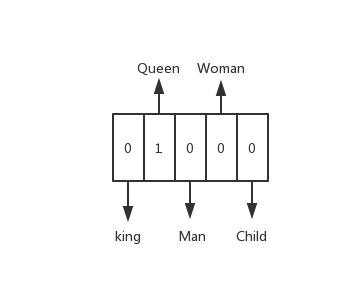
\includegraphics[width=0.4\textwidth]{img/fig8.png}
  \caption{one hot representation}
  \label{figure:zju6}
  \end{figure}

One hot representation用来表示词向量非常简单,但是却有很多问题。最大的问题是我们的词汇表一般都非常大,比如达到百万级别,这样每个词都用百万维的向量来表示简直是内存的灾难。

Dristributed representation可以解决One hot representation的问题,它的思路是通过训练,将每个词都映射到一个较短的词向量上来。所有的这些词向量就构成了向量空间,进而可以用普通的统计学的方法来研究词与词之间的关系。这个较短的词向量维度是多大呢?这个一般需要我们在训练时自己来指定。

比如下图我们将词汇表里的词用"Royalty","Masculinity", "Femininity"和"Age"4个维度来表示,King这个词对应的词向量可能是(0.99,0.99,0.05,0.7)。当然在实际情况中,我们并不能对词向量的每个维度做一个很好的解释。

\begin{figure}[htbp]
  \centering
  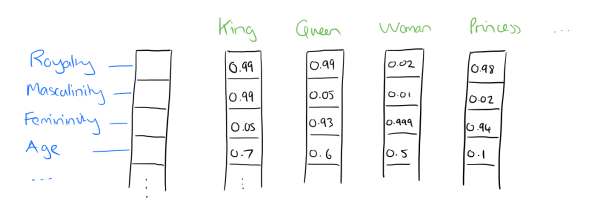
\includegraphics[width=0.4\textwidth]{img/fig9.png}
  \caption{Dristributed representation}
  \label{figure:zju7}
  \end{figure}

CBOW模型的训练输入是某一个特征词的上下文相关的词对应的词向量,而输出就是这特定的一个词的词向量。比如下面这段话,我们的上下文大小取值为4,特定的这个词是"Learning",也就是我们需要的输出词向量,上下文对应的词有8个,前后各4个,这8个词是我们模型的输入。由于CBOW使用的是词袋模型,因此这8个词都是平等的,也就是不考虑他们和我们关注的词之间的距离大小,只要在我们上下文之内即可。

\begin{figure}[htbp]
  \centering
  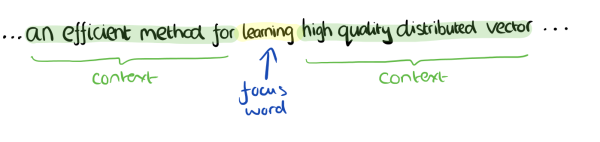
\includegraphics[width=0.4\textwidth]{img/fig10.png}
  \caption{one hot representation}
  \label{figure:zju8}
  \end{figure}

这样我们这个CBOW的例子里,我们的输入是8个词向量,输出是所有词的softmax概率(训练的目标是期望训练样本特定词对应的softmax概率最大),对应的CBOW神经网络模型输入层有8个神经元,输出层有词汇表大小个神经元。隐藏层的神经元个数我们可以自己指定。通过DNN的反向传播算法,我们可以求出DNN模型的参数,同时得到所有的词对应的词向量。这样当我们有新的需求,要求出某8个词对应的最可能的输出中心词时,我们可以通过一次DNN前向传播算法并通过softmax激活函数找到概率最大的词对应的神经元即可。

% 余弦相似度不再详述。

\subsubsection{训练模型及相似度比较步骤}
1.基于预处理的文本,建立词向量,采用$CBOW$训练神经网络,优化收敛词向量;

2.依据短文本中各个关键词的tfidf权重,将短文本中包含的词向量做加权平均,作为该短文本的词向量;

3.比较两个短文本向量的COS相似度。

\subsection{metadata其他数据对比}
\subsubsection{字符串相似度}
1.选取$metadata$中的$title$、$package\_name$、$developer\_email$等字段;

2.采用字符串的编辑距离度量相似度。

\subsubsection{特征向量相似度}
1.选取$metadata$中的$app\_category$、$app\_type$、$permission$等字段;

2.建立词汇表,取词汇表下标并进行归一化,将最后所得数值作为特征向量;

3.计算特征向量间的余弦相似度。

\subsection{$apk\_icon$对比——感知哈希算法}
对每张图片生成一个"指纹"(fingerprint)字符串,然后比较不同图片的指纹。结果越接近,就说明图片越相似。步骤如下:

1. 第一步,缩小尺寸。将图片缩小到8x8的尺寸,总共64个像素。这一步的作用是去除图片的细节,只保留结构、明暗等基本信息,摒弃不同尺寸、比例带来的图片差异。

2.第二步,简化色彩。将缩小后的图片,转为64级灰度。也就是说,所有像素点总共只有64种颜色。

3.第三步,计算平均值。计算所有64个像素的灰度平均值。

4. 第四步,比较像素的灰度。将每个像素的灰度,与平均值进行比较。大于或等于平均值,记为1;小于平均值,记为0。

5. 第五步,计算哈希值。将上一步的比较结果,组合在一起,就构成了一个64位的整数,这就是这张图片的指纹。组合的次序并不重要,只要保证所有图片都采用同样次序就行了。

得到指纹以后,就可以对比不同的图片,看看64位中有多少位是不一样的。理论上,这等同于计算汉明距离($Hamming distance$)。如果不相同的数据位不超过5,就说明两张图片很相似;如果大于10,就说明这是两张不同的图片。

\section{成果展示}
\subsection{metadata数据对比}
选取$metadata$中的$description\_html$字段,对比如图\ref{figure:zju1}和\ref{figure:zju2}所示:

\begin{figure}[htbp]
\centering
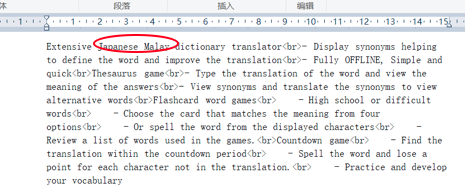
\includegraphics[width=0.2\textwidth]{img/fig1.png}
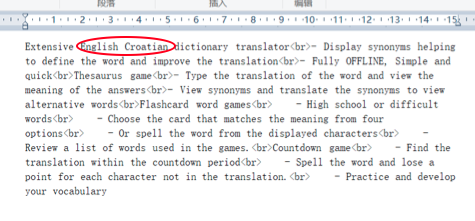
\includegraphics[width=0.2\textwidth]{img/fig2.png}
\caption{相似度为0.999999963的两段文本对比}
\label{figure:zju1}
\end{figure}

\begin{figure}[htbp]
  \centering
  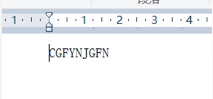
\includegraphics[width=0.2\textwidth]{img/fig3.png}
  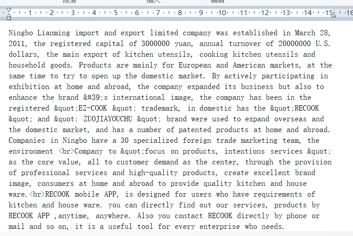
\includegraphics[width=0.2\textwidth]{img/fig4.png}
  \caption{相似度为0.173356448的两段文本对比}
  \label{figure:zju2}
  \end{figure}

选取$metadata$中的$title$、$package\_name$、$developer\_email$等字段,对比如图\ref{figure:zju3}、图\ref{figure:zju4}和图\ref{figure:zju5}所示:

\begin{figure}[htbp]
  \centering
  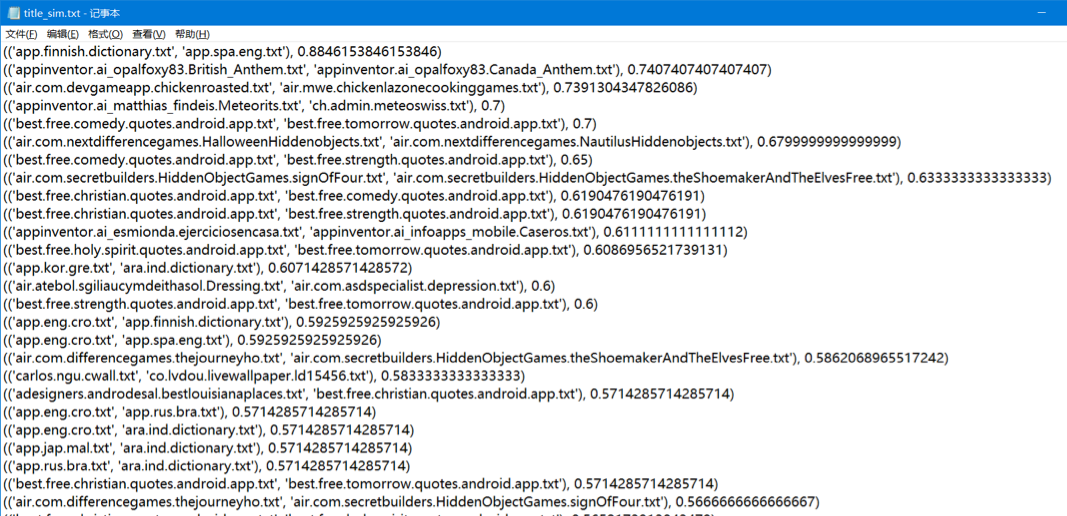
\includegraphics[width=0.4\textwidth]{img/fig5.png}
  \caption{title字段的相似度对比}
  \label{figure:zju3}
  \end{figure}

\begin{figure}[htbp]
  \centering
  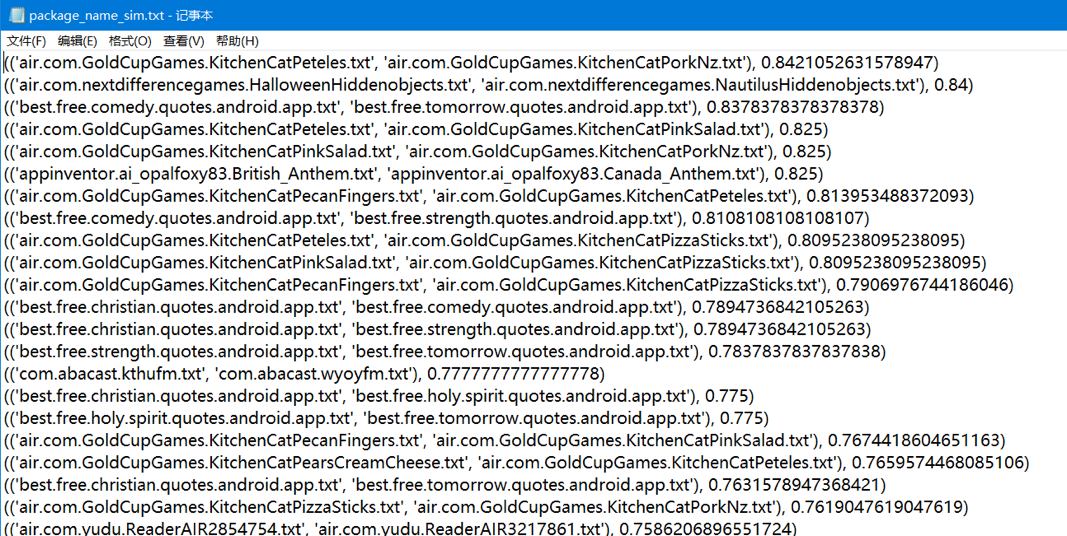
\includegraphics[width=0.4\textwidth]{img/fig6.png}
  \caption{$package\_name$字段相似度对比}
  \label{figure:zju4}
  \end{figure}

\begin{figure}[htbp]
  \centering
  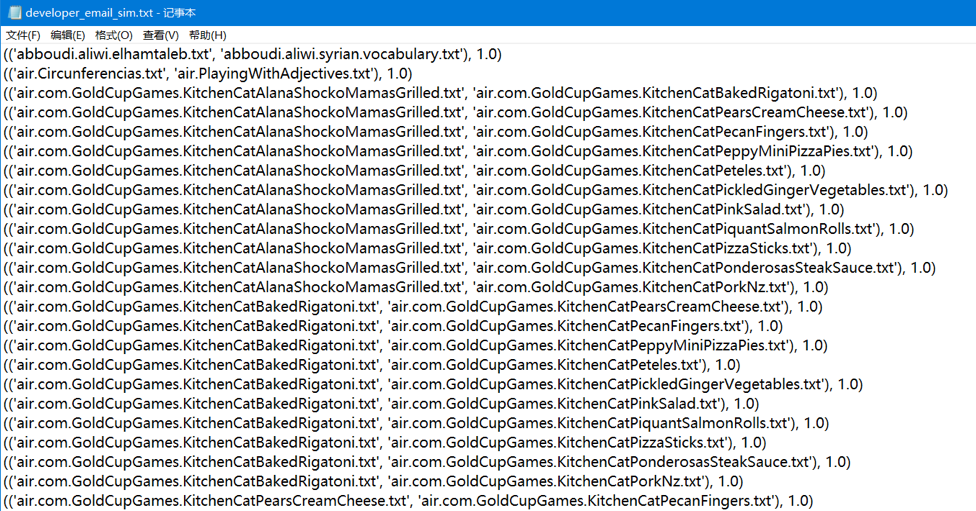
\includegraphics[width=0.4\textwidth]{img/fig7.png}
  \caption{$developer\_email$字段相似度对比}
  \label{figure:zju5}
  \end{figure}

\subsection{$apk\_icon$数据对比}
对每张图片生成一个“指纹”(fingerprint)字符串,然后比较不同图片的指纹。结果越接近,就说明图片越相似,对比如图\ref{figure:zju9}和图\ref{figure:zju10}所示。

\begin{figure}[htbp]
  \centering
  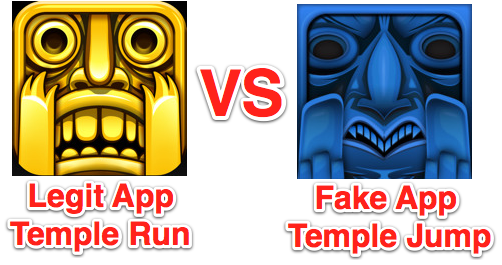
\includegraphics[width=0.4\textwidth]{img/fig11.png}
  \caption{汉明距离为9的$app\_icon$对比}
  \label{figure:zju9}
  \end{figure}

\begin{figure}[htbp]
  \centering
  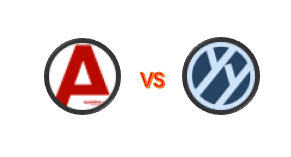
\includegraphics[width=0.4\textwidth]{img/fig12.png}
  \caption{汉明距离为35的$app\_icon$对比}
  \label{figure:zju10}
  \end{figure}

\section{总结}
本作品通过分析目前国内外典型恶意应用软件的实现原理,采用两种方式对应用软件进行检测。通过实验验证,本作品的仿冒App检测方案有一定的可行性与有效性,取得了较理想的效果,但是还是有一些缺陷以及不足:(1)样本库数据量较小;(2)图片指纹数据量大,算法运行速度慢;

通过一个多月的努力,本作品也已经逐渐完善,感谢王浩宇老师给我们提供了这样一个机会,期间我们从无到有,看到的多,学到的也更多,包括如何查询有效的信息,如何快捷地学到我们想学的知识。
在未来的研究中,还需要对本作品进行进一步的完善,探索精度更高、运行速度更快的检测算法。

\section{致谢}
感谢学校提供的学习与实践的机会;感谢王浩宇老师给予的耐心指导;

\end{document}